\section{Design of an FPGA-based accelerator integrating structured sparse DSC} \label{sec:design}
%
As previously said, this section aims at developing a pruning scheme for the \acrshort{dsc} that fulfills the proposed design objectives and an algorithm able to support it. First, we detail the pruning scheme used and the weight and operation reduction factors obtained when applying the pruning scheme. Second, we analyze the sparse kernels to find a compressed format that reduces memory usage and overhead of determining the address of the non-pruned weights. Third, we describe the algorithm proposed to perform the sparse \acrshort{dsc} using the proposed pruning scheme. Finally, we analyze the convolution loops to determine the optimal design of the \acrshort{pe} that performs the convolution.
%
\subsection{Pruning scheme} \label{subsec:pscheme}
%
\acrshort{dsc} is composed of two types of convolution: depthwise and pointwise convolutions (see Section \ref{subsec:layer}). We decided to apply pruning on the pointwise filters for the following reasons:
%
\begin{itemize}
    \item In MobileNet and MobileNetV2, most of the operations are done in the pointwise convolutions \cite{zhang_channel_2019, tu_pruning_2019}. So it is the operation where the reduction of weights and computational complexity would be the most relevant (each operation requires one weight).
    \item As each kernel of a pointwise filter is a vector of size $1 \times 1  \times N_{if}$, we, therefore, have to prune in the channel-axis. This scheme was proven to be successful by \textcite{kang_accelerator-aware_2020}.
    \item The pruning scheme can be applied to each $1 \times 1$ convolution of the network.
\end{itemize}
%
As mentioned above, we decided to develop a pruning scheme inspired by the methodology of \textcite{kang_accelerator-aware_2020}, which prunes weights in the channel-axis.

Ideally, without pruning, each \acrshort{pe} performing a pointwise convolution fetches $N_{if}$ weights and input pixels corresponding to spatial coordinates $(x, y)$ in each input channel (pointwise convolution only convolves pixels in the channel-axis). Then each weight is multiplied with its corresponding pixel and the products are summed to obtain one output pixel of one channel. If we apply an unstructured pruning on the pointwise filter, we can use the same algorithm as above but only each non-pruned weight is multiplied with its corresponding pixel (multiplication implying zero-value weights can be safely discarded).

However, as the resources of the \acrshort{fpga} are limited, the \acrshort{pe} can only fetch $N_{par} \leq N_{if}$ weights and pixels at each time (which corresponds to a \textbf{fetching group}; each input \acrshort{fm} and kernel are composed of $N_{gr}$ fetching groups). Therefore, we would do the convolution between each fetching group and accumulate the different partial sums belonging to the same output pixel until an output pixel is produced. If an unstructured pruning is applied, this can cause several issues, as pointed out by \cite{kang_accelerator-aware_2020}.

First, it can cause misalignment between the weight and pixel fetching groups. Indeed if we prune the first $N_{par}$ weights in the kernel, the first pixel fetching group is useless. Second, there can be a load-imbalance problem (see Section \ref{subsec:impl_prun}) that can occur between two \acrshort{pe}s if the number of pruned weights between two kernels is different. 

To solve these problems, the solution proposed by \textcite{kang_accelerator-aware_2020} is to align pixel and weight fetching groups. Each pixel fetching group has a corresponding weight fetching group containing at least one non-pruned weight. \textcite{kang_accelerator-aware_2020} also constrains the number of non-pruned weights in each fetching group to be the same number, called $N_{np}$. Therefore, it solves also the load-imbalance problem. As a result, the proposed sparse \acrshort{dsc} can be illustrated in Figure \ref{fig:prunedwg}.
%
\begin{figure}[H]
    \centering
    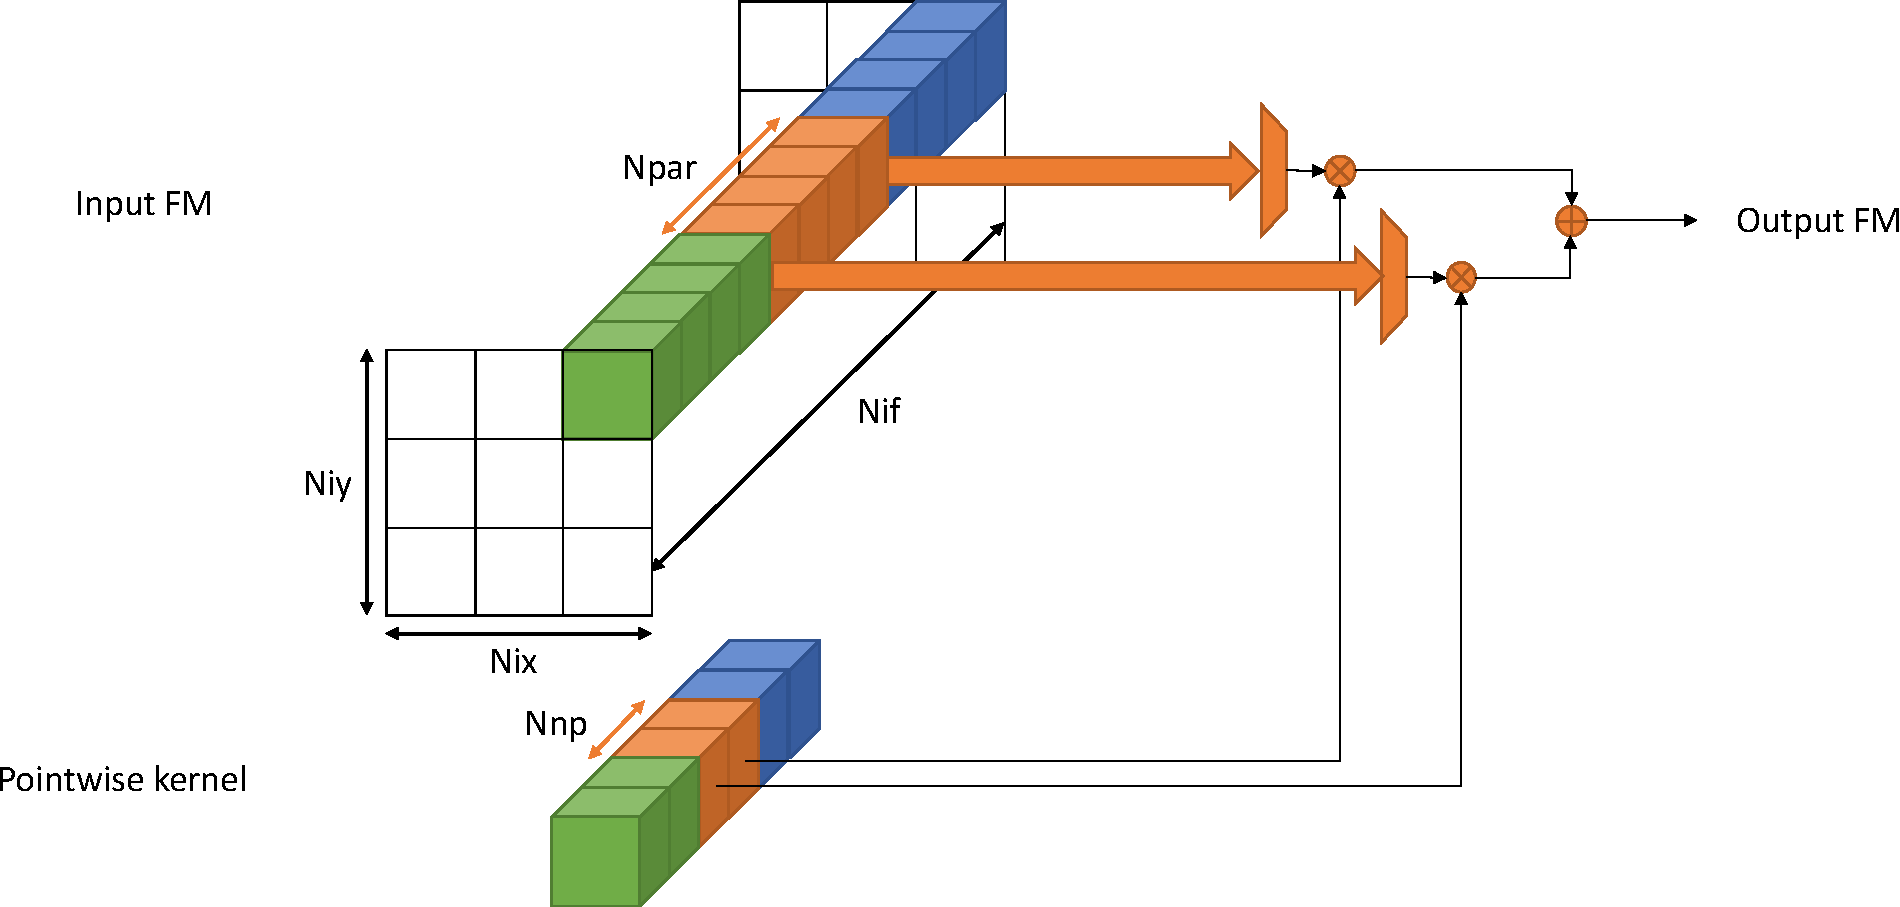
\includegraphics[width=\textwidth]{pruningscheme.pdf}
    \caption{Process of a pointwise convolution with a sparse pointwise kernel, where $N_{par} = 4$ and $N_{np} = 2$, inspired by \cite{kang_accelerator-aware_2020}}
    \label{fig:prunedwg}
\end{figure}
%
To summarize, each pointwise kernel is composed of $N_{gr}$ fetching groups of $N_{np}$ weights. Each group corresponds to a pixel fetching group of size $N_{par}$. We define the ratio between the number of non-pruned weights and the size of the fetching group without pruning as the \textbf{pruning ratio $\alpha$}, in other words, the ratio of weights remaining after pruning. The ratio of pruned weights is therefore equal to $1 - \alpha$. The pruning parameters are defined in Table \ref{tab:pr_param}. Moreover, the proposed pruning scheme can also be applied to each $1 \times 1$ kernel.
%
\begin{table}[H]
    \center
    \begin{tabular}{|c|c|c|}
        \hline
        $N_{par}$ & The input pixel fetching group size. & $N_{par} \leq N_{if}$ \\
        \hline
        $N_{np}$  & The pointwise weight fetching group size. & $N_{np} \leq N_{par}$ \\
        \hline
        $N_{gr}$  & The number of fetching groups & $N_{gr} = \left\lceil \frac{N_{if}}{N_{par}} \right\rceil $ \\
        \hline
        $\alpha$  & The pruning ratio & $\alpha = \frac{N_{np}}{N_{par}}  $ \\
        \hline
    \end{tabular}
    \caption{Pruning parameters}
    \label{tab:pr_param}
\end{table}
%
We should add that this pruning scheme is not the same as \textit{channel pruning} since we do not constrain the same weights to be pruned in each group. Therefore, I did not consider the pruning of the depthwise kernel associated with the pruning of weight in each kernel, as discussed in Section \ref{subs:pruning}. We proposed then a pruning-scheme that is not coarse-grained (channel pruning), satisfying first design objective: \textbf{\textquote{The pruning scheme is as fine-grained as possible}}.
%
\subsubsection{Reduction factors}
%
We can now evaluate the reduction factors of the sparse \acrshort{dsc} compared with the \acrshort{dsc} without pruning, and with the standard convolution. We consider that the size of the input feature map is $N_{ix}  \times N_{iy} \times N_{if}$, the size of the depthwise filter is $N_{kx} \times N_{ky} \times N_{if}$, the size of the non-pruned pointwise convolution $N_{if} \times N_{of}$, the fetching group size is $N_{par}$, the number of pruned weights is $N_{np}$, and the size of the output \acrshort{fm} is $N_{ox}  \times N_{oy} \times N_{of}$. 

The number of weights $W_{DSC}$ and operations $O_{DSC}$ of the \acrshort{dsc} can be determined using Equation \eqref{eq:dsc_wg} and \eqref{eq:dsc_op} \cite{liu_fpga-based_2019, bai_cnn_2018}.
%
\begin{equation}
    W_{DSC} = N_{kx} \times N_{ky} \times N_{if} + N_{if} \times N_{of}
    \label{eq:dsc_wg}
\end{equation}
%
\begin{equation}
    O_{DSC} = N_{ix} \times N_{iy} \times N_{kx} \times N_{ky} \times N_{if} + N_{ix} \times N_{iy} \times N_{if} \times N_{of}
    \label{eq:dsc_op}
\end{equation}

In the same manner, the amount of weights $W_{PR\_DSC}$ and operations $O_{PR\_DSC}$ of the sparse \acrshort{dsc} can be determined using Equation \eqref{eq:pr_dsc_wg} and \eqref{eq:pr_dsc_op}.
%
\begin{equation}
    W_{PR\_DSC} = N_{kx} \times N_{ky} \times N_{if} + N_{np} \times N_{gr} \times N_{of}
    \label{eq:pr_dsc_wg}
\end{equation}
%
\begin{equation}
    O_{PR\_DSC} = N_{ix} \times N_{iy} \times N_{kx} \times N_{ky} \times N_{if} + N_{ix} \times N_{iy} \times N_{gr} \times N_{np} \times N_{of}
    \label{eq:pr_dsc_op}
\end{equation}

Thus, the weights $F_{Wg}$ and operations $F_{Op}$ reduction factors can be expressed according to Equation \eqref{eq:factor_comp_wg} and \eqref{eq:factor_comp_op}. The demonstration allowing to find these relations can be found in Appendix \ref{appendix:factor}.
%
\begin{equation}
    F_{Wg} = \frac{W_{DSC}}{W_{PR\_DSC}} = \frac{1 + \frac{N_{kx} \times N_{ky}} {N_{of}}} {\alpha + \frac{N_{kx} \times N_{ky}} {N_{of}}}
    \label{eq:factor_comp_wg}
\end{equation}
\begin{equation}
    F_{Op} = \frac{O_{DSC}}{O_{PR\_DSC}} = \frac{1 + \frac{N_{kx} \times N_{ky}} {N_{of}}} {\alpha + \frac{N_{kx} \times N_{ky}} {N_{of}}}
    \label{eq:factor_comp_op}
\end{equation}

As the reduction factors depend on the pruning ratio $\alpha$ and the number of output channels $N_{of}$, we can illustrate the evolution of the reduction factors depending on $\alpha$ and the different $N_{of}$ of MobileNetV2, as shown in Figure \ref{fig:redfacto}.
%
\begin{figure}[H]
    \centering
    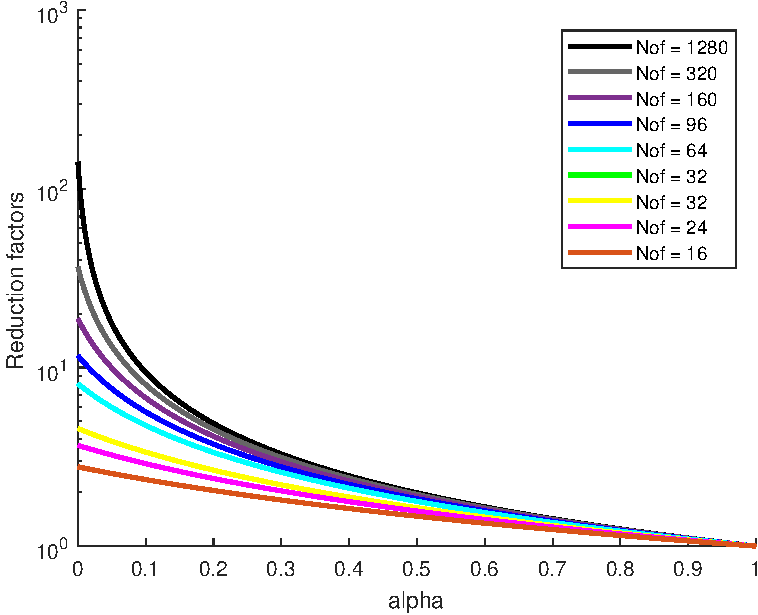
\includegraphics[width=0.75\textwidth]{RedFactor.pdf}
    \caption{Evolution of the reduction factors depending on the pruning ratio and the number of output channels}
    \label{fig:redfacto}
\end{figure}

For example, if we apply a pruning ratio of $25\%$ (meaning keeping $25\%$ of the weights in each fetching group), the reduction factors compared to the \acrshort{dsc} without pruning are between two and four times. If we consider the reduction factor between \acrshort{dsc} and standard convolution is about 9 times \cite{zhang_channel_2019}, the reduction factors between sparse \acrshort{dsc} and standard convolution is between 18 and 36 times (if $\alpha = 25\%$). We, therefore, validated the second design objective: \textbf{\textquote{The pruning scheme reduces the computational complexity}}.
%
\subsection{Compressed format} \label{subs:compress_f}
%
After applying the pruning scheme on the pointwise kernels, these kernels become sparse. This means that they contain zero-value weights, as illustrated in Figure \ref{fig:pruned_wg}. Therefore, to reduce memory usage, we should only store each non-pruned weight in a compressed format that allows finding its address with no extra-overhead.
%
\begin{figure}[H]
    \centering
    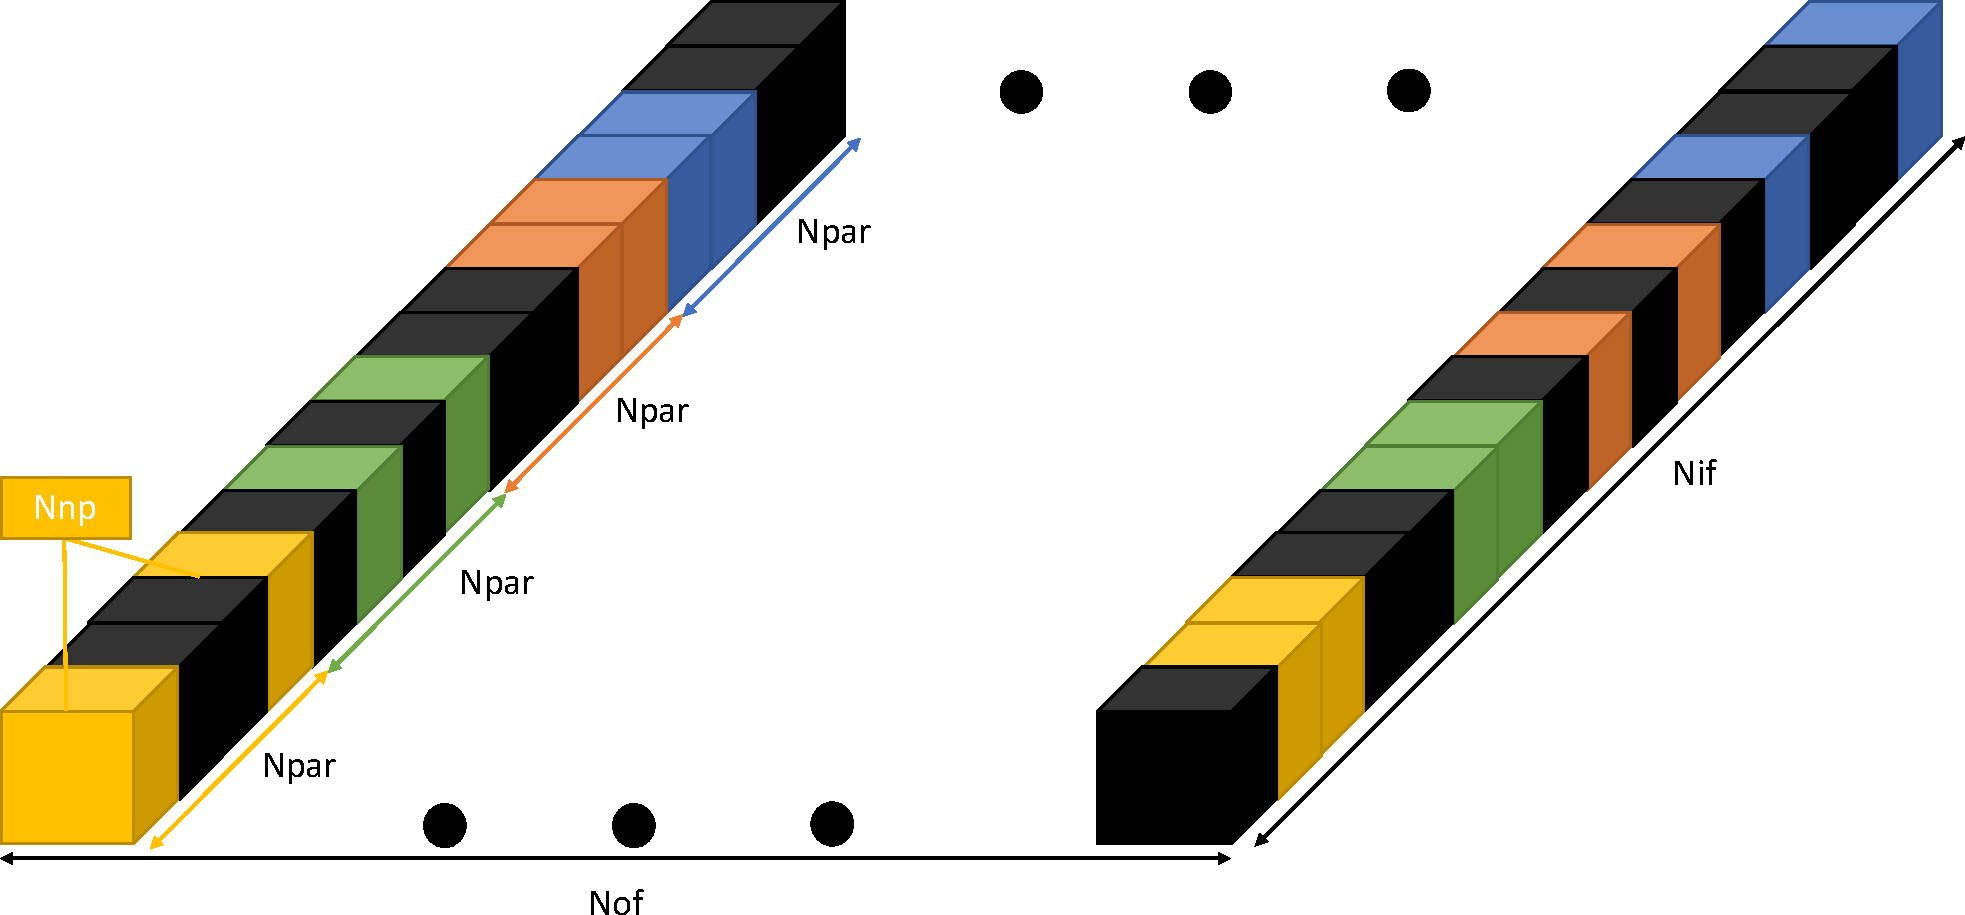
\includegraphics[width=0.75\textwidth]{pruned_wg.pdf}
    \caption{A pointwise kernel after pruning, where black cubes are pruned weights}
    \label{fig:pruned_wg}
\end{figure}

A conventional storage format for a sparse matrix is the \acrfull{csr} \cite{buluc_parallel_2009}. According to \textcite{buluc_parallel_2009}, \textquote{\textit{The compressed sparse row (CSR) format stores the nonzeros (and ideally only the nonzeros) of each matrix row in consecutive memory locations,  and  it  stores  an  index  to  the  first  stored  element of each row}}. In other words, we can represent a sparse matrix using three vectors:
%
\begin{itemize}
    \item \textbf{Vector val}: containing all the values of the non-pruned weights.
    \item \textbf{Vector col\_ind}: containing the column indices of the elements in \textbf{val}.
    \item \textbf{Vector row\_ptr}: containing the index of each row in \textbf{val}.
\end{itemize}
%
However, as for \cite{zhu_efficient_2020}, the \acrshort{csr} format can be compressed further thanks to the pruning scheme applied. Indeed, since the kernels to compress are vectors, we can reduce the storage usage by removing the \textbf{row\_ptr} vector (the kernel has only one row). 

Moreover, we can have a better compression if we reduce the number of bits allocated to represent the column index of a weight. Indeed, as each weight corresponds to an input fetching group of size $N_{par}$, it is sufficient to store the position of the weight in that group, instead of its absolute position in the kernel. As a result, we can reduce the number of bits from $log_2(N_{if})$ (absolute position) to $log_2(N_{par})$ (relative position), where $N_{par} \leq N_{if}$. Moreover, it also reduces the overhead to find the corresponding pixel in a fetching group, for each weight.

In brief, each sparse kernel is converted into 2 vectors of size $N_{np}$: vector \textbf{val}, which contains the value of the non-pruned weights, and vector \textbf{position}, which contains the position of the corresponding pixel in a fetching group. An example is illustrated in figure \ref{fig:compressed_format}.
%
\begin{figure}[H]
    \centering
    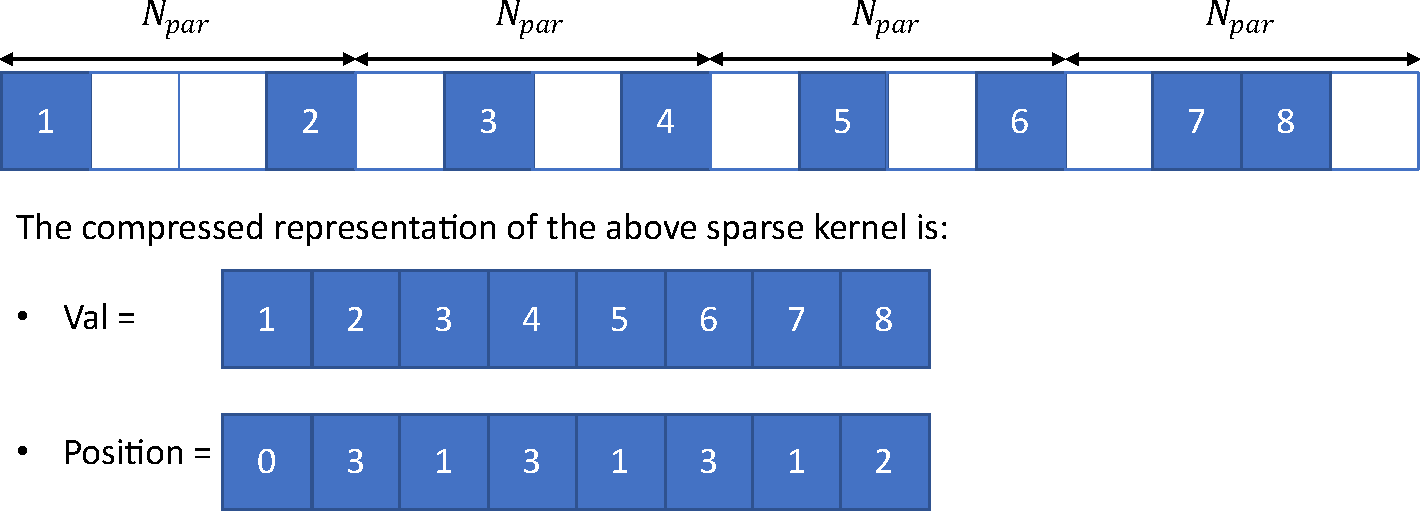
\includegraphics[width=0.75\textwidth]{compressed_format.pdf}
    \caption{Illustration of the compressed format, where $N_{par} = 4$ and $N_{np} = 2$}
    \label{fig:compressed_format}
\end{figure}

Since this compressed format requires storing the value and the position of each weight (and hence more bits allocated per weight), we computed the maximal pruning ratio, or in the same way, the minimal ratio of pruned weights, required to have a reduction of memory usage. The relation between maximal pruning ratio and memory reduction can be found in Equation \eqref{eq:prun_mem} where $BW_{weight}$ is the bitwidth required to represent the value of a weight. The demonstration to find the maximal pruning ratio $\alpha$ to reduce memory usage can be found in Appendix \ref{appendix:cf}.
%
\begin{equation}
    \alpha < \frac{BW_{weight}}{ BW_{weight} + log_2(N_{par})}
    \label{eq:prun_mem}
\end{equation}

The curve representing the minimal ratio of pruned weight, equals to $1 - \alpha$, depending on $N_{par}$ when $BW_{weight} = 16$ is illustrated in Figure \ref{fig:prun_mem}. We can conclude from the curve that we need to have a ratio of pruned weights to be greater or equal than $40\%$ to save memory. We can also conclude that we can prune fewer weights if we reduce the value of $N_{par}$. 

We, therefore, validated the third design objective, which is: \textbf{\textquote{The pruning scheme allows a reduction of the memory required to store the weights}}.
%
\begin{figure}[H]
    \centering
    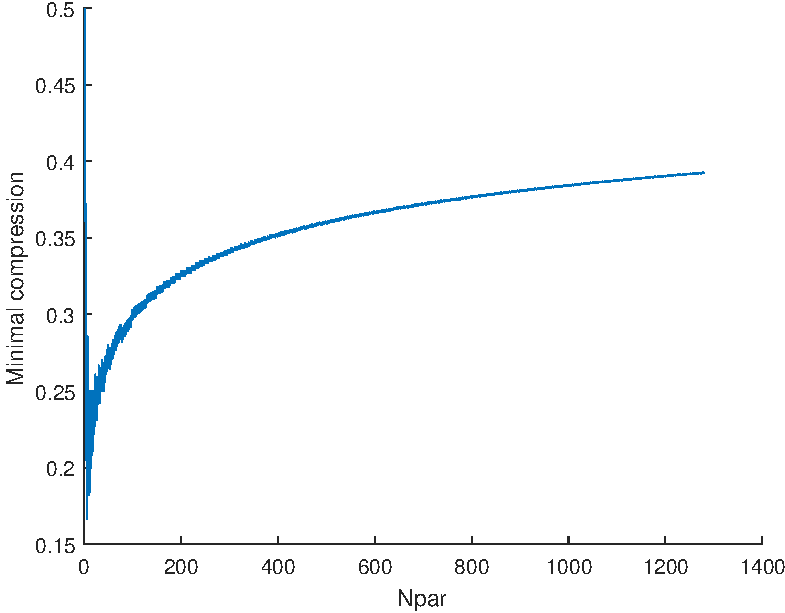
\includegraphics[width=0.70\textwidth]{MinCompr.pdf}
    \caption{Minimal ratio of pruned weights if $BW$ = 16}
    \label{fig:prun_mem}
\end{figure}
%
\subsection{Adding the pruning scheme to MobileNetV2} \label{subsec:mbnv2-pr}
%
As we have seen how the weights of a $1 \times 1$ kernel are pruned and explained the compressed format of the kernels, we present in this section how to integrate the proposed pruning scheme into MobileNetV2. In MobileNetV2, the \acrshort{dsc} layer is included in a larger building block, the \textit{Bottleneck residual block} which performs the bottleneck convolution (see Section \ref{subs:mbv2}). In the bottleneck convolution, the \acrshort{dsc} follows a $1 \times 1$ convolution layer that expands the number of input channels by a factor t. As a result, we have to compute two sparse $1 \times 1$ convolutions. We note that the \acrshort{fm} produced by the $1 \times 1$ convolution is referenced as \textbf{intermediate \acrshort{fm}} in the rest of this thesis. The intermediate \acrshort{fm} is composed of $N_{gr_{int}} = t \times N_{gr}$ fetching groups, which are fed to the \acrshort{dsc}.

As explained in Section \ref{subsec:pscheme}, each $1 \times 1$ and pointwise convolutions have to fetch $N_{par}$ input pixels in the channel-axis, which corresponds to $N_{par}$ channels. Consequently, if the $1 \times 1$ convolution produces $N_{par}$ channels, the \acrshort{dsc} can fetch those intermediate products to produce partial results of the output \acrshort{fm}. Indeed, we can perform the depthwise convolution with each intermediate channel and then perform the pointwise convolution with the corresponding weight in each pointwise kernel, as illustrated in Figure \ref{fig:algo}. The output \acrshort{fm} is computed when the \acrshort{dsc} has performed these steps for each intermediate group.
%
\begin{figure}[H]
    \centering
    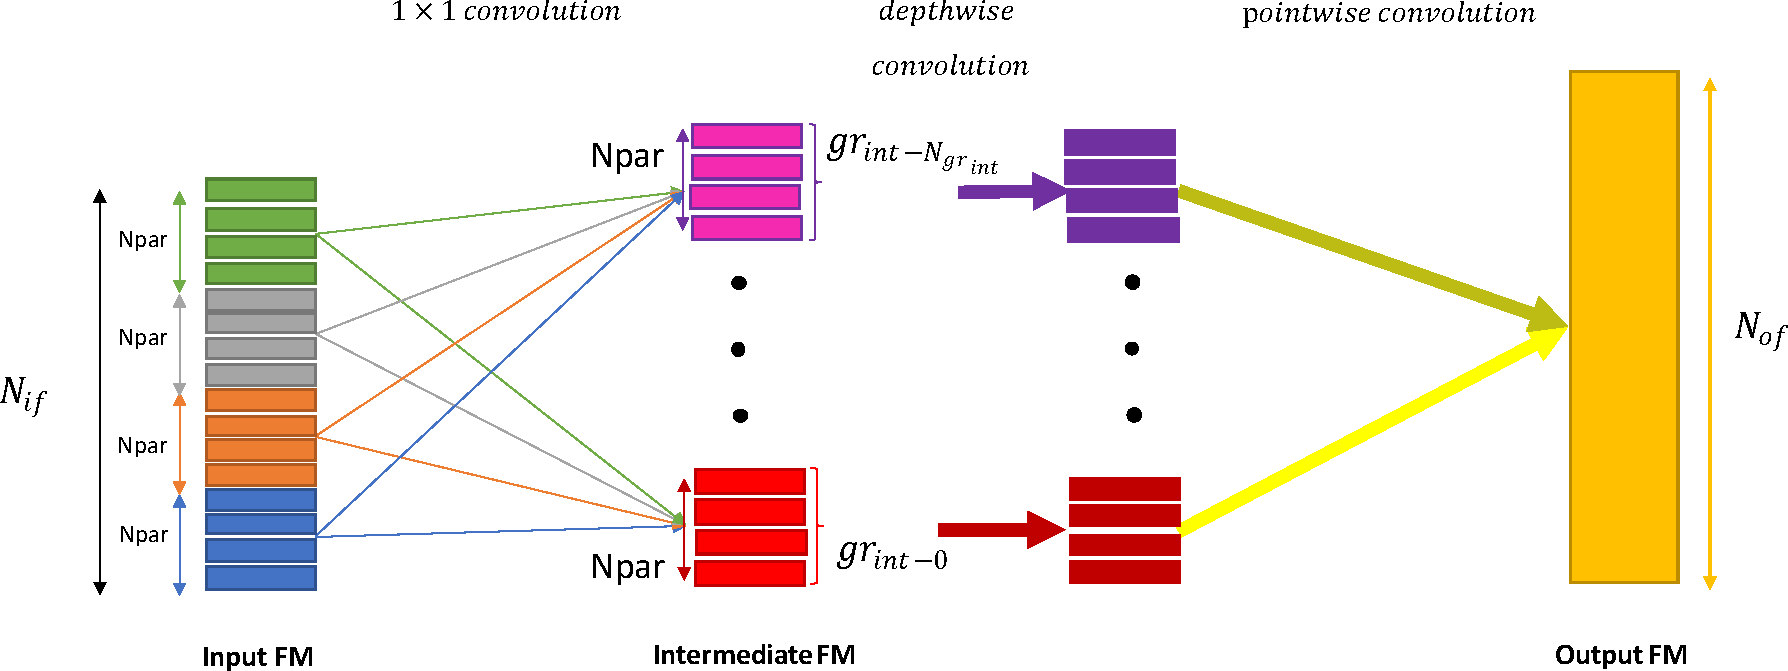
\includegraphics[width=\textwidth]{algo.pdf}
    \caption{Illustration of the algorithm used to perform the convolutions}
    \label{fig:algo}
\end{figure}

This approach was chosen, instead of producing directly each final output result, to reuse at most the products of the $1 \times 1$ convolution. Indeed, if we aim at directly producing a final output, the $1 \times 1$ convolution has to produce $N_{kx} \times N_{ky} \times N_{ky} \times N_{par}$ intermediate results. When the \acrshort{dsc} has computed the partial sum from this fetching group (for one kernel since we prioritize the computation of one final pixel), the old intermediate pixels will be overwritten by the next fetching group intermediate pixels, which could have been reused for another pointwise kernel.

We can translate this algorithm into pseudocode, observed in Algorithm \ref{pseudocode:overal_pseudo_code}, where $group$ (respect. $group_{int}$) is the index of the fetching group in the input \acrshort{fm} (resp. intermediate \acrshort{fm}) and $Ngr_{int} = \left\lceil \frac{N_{if} \times t}{N_{par}} \right\rceil$ is the number of intermediate fetching groups. The detailed algorithm to perform each convolution can be described as follow:
\begin{algorithm}[H]
    \centering
    \begin{algorithmic}
        \For{$group_{int}:=0$; $group_{int} < Ngr_{int}$; $group_{int}++$}
            \State{$1 \times 1$ convolution ($group_{int}$)}
            \State{DSC($group_{int}$);}
        \EndFor
    \end{algorithmic}
    \caption{Pseudocode of the algorithm}
    \label{pseudocode:overal_pseudo_code}
\end{algorithm}
%
\begin{enumerate}
    \item \textbf{$1 \times 1$ convolution}: We must fetch the $N_{par}$ kernels corresponding to the \acrshort{dsc} fetching group $group_{int}$. Indeed, the \acrshort{dsc} needs to fetch $N_{par}$ channels of the intermediate \acrshort{fm} (each kernel produces one channel). Then we can perform the convolution with the input \acrshort{fm}. As described in Section \ref{subs:2dconv}, the kernel acts like a sliding window on the input \acrshort{fm}. For each pixel at position $(ix, iy)$, the convolution loads iteratively each weight and pixel fetching group in the channel-axis. For each fetching group $group \leq N_{group}$, the convolution is performed by multiplying each non-pruned weight with its corresponding pixel and accumulates the multiplication with the result of the previous group. The process is finished when the $N_{par}$ intermediate \acrshort{fm} channels have been produced (of size $N_{ix} \times N_{iy}$). The corresponding pseudocode is found in Algorithm \ref{pseudocode:c11} and the process is shown in Figure \ref{fig:algo_11conv}.
    \begin{algorithm}[H]
        \centering
        \begin{algorithmic}
            \For{$int_{f}:=0$; $int_{f} < N_{par}$; $int_{f}++$} \Comment{Loop 3}
                \For{$int_{x}:=0$; $int_{x} < N_{ix}$; $int_{x}++$} \Comment{Loop 2}
                    \For{$int_{y}:=0$; $int_{y} < N_{iy}$; $int_{y}++$} \Comment{Loop 2}
                        \For{$group:=0$; $group < N_{gr}$; $group++$} \Comment{Loop 1}
                            \For{$i_f:=0$; $i_f < N_{np}$; $i_f++$} \Comment{Unrolled}
                                \State{$wgt$  = $filter_{1 \times 1}$[$group_{int} \times N_{par} + int_f$][$group \times N_{np} + i_f$]}
                                \State{$acti$  = $FMI_{I}$[$wgt[pos] + group \times N_{par}$][$int_y$][$int_x$]}
                                \State{FM$_{int}$[$group_{int} \times N_{par} + int_f$][$int_y$][$int_x$]  += $acti \times wgt[val]$}
                            \EndFor
                        \EndFor
                    \EndFor
                \EndFor
            \EndFor
        \end{algorithmic}
        \caption{Sparse $1 \times 1$ convolution pseudocode}
        \label{pseudocode:c11}
    \end{algorithm}
    %
    \begin{figure}[H]
        \centering
        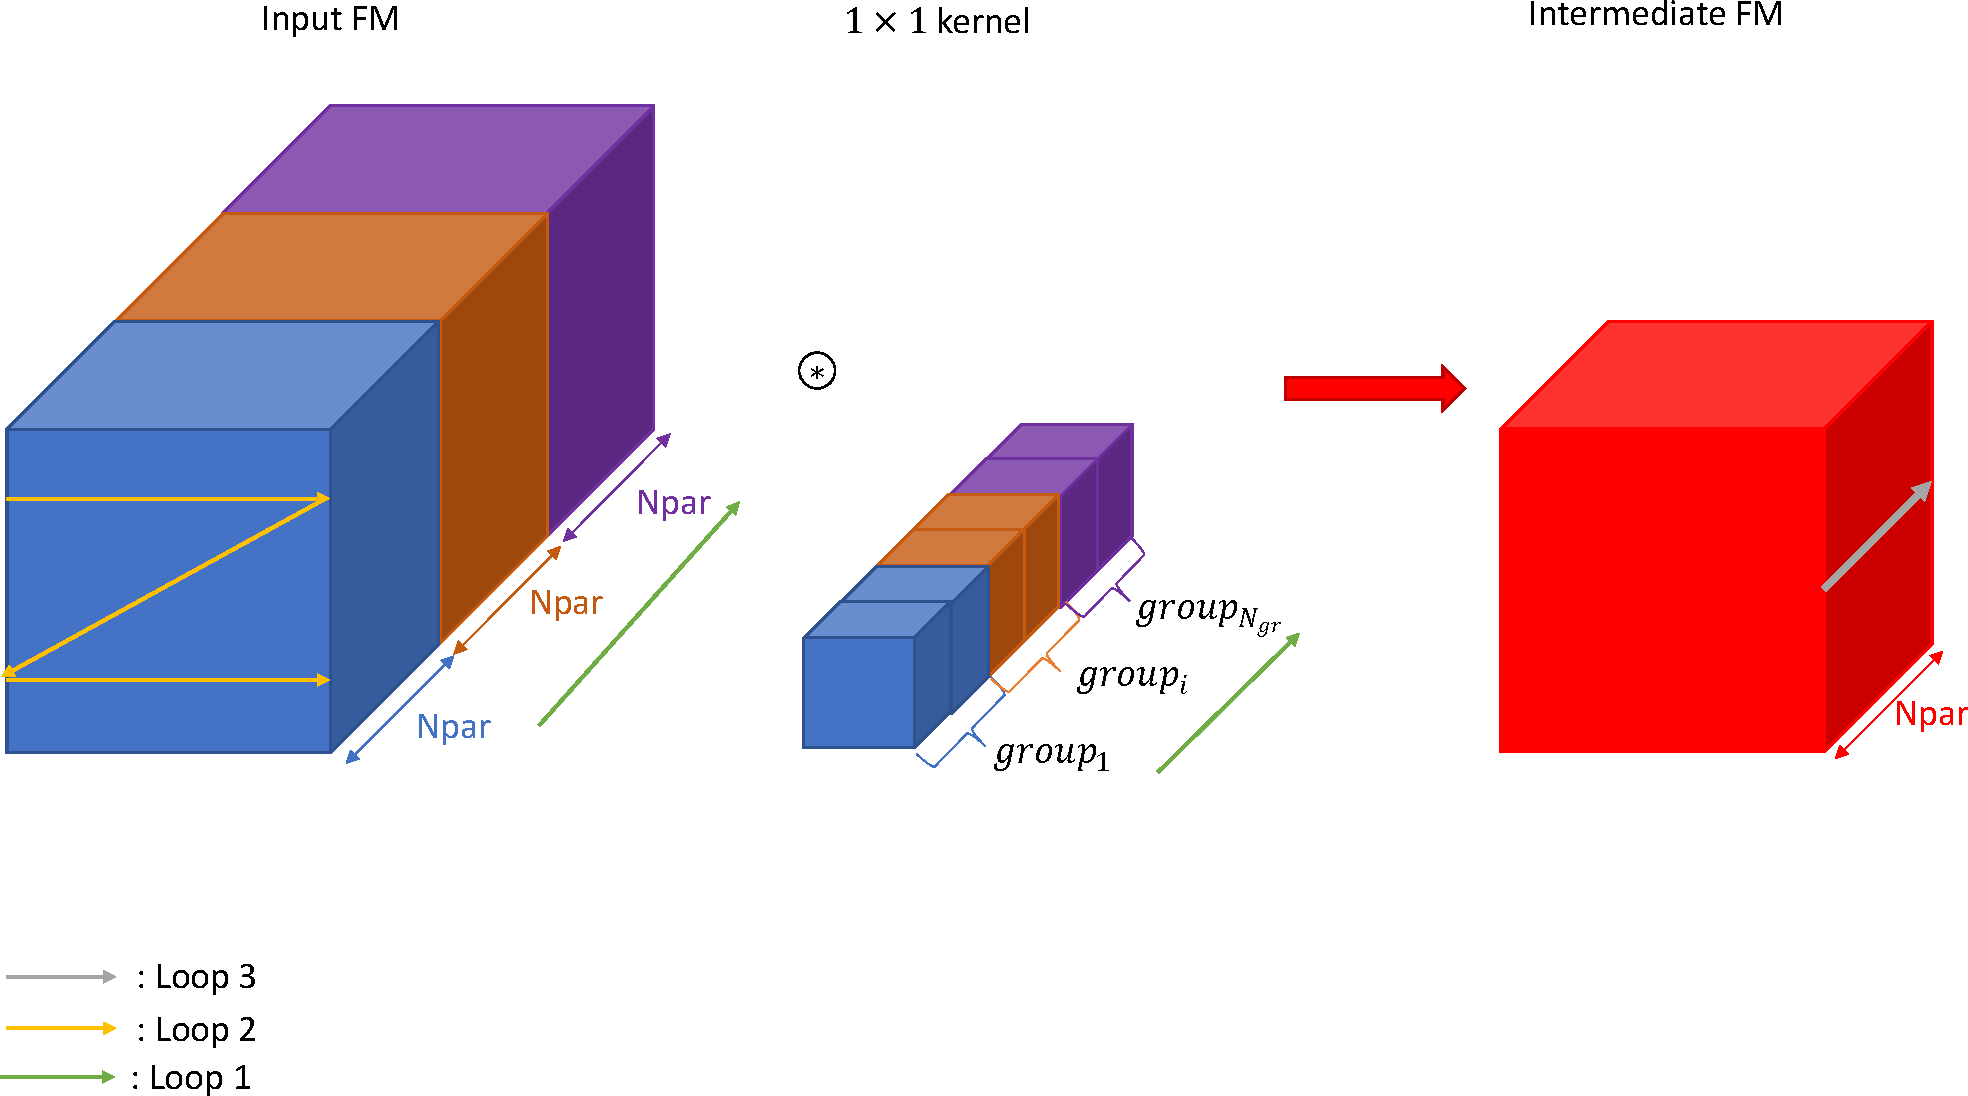
\includegraphics[width=0.75\linewidth]{algo_c11.pdf}
        \caption{Representation of the sparse $1 \times 1$ convolution}
        \label{fig:algo_11conv}
    \end{figure}
    %
    \item \textbf{\acrshort{dsc}}: Once the $1 \times 1$ convolution has produced the next $N_{par}$ intermediate \acrshort{fm} channels, we can do the depthwise convolution with these channels. The depthwise convolution first computes the 2D convolution of each of the intermediate \acrshort{fm} channels. Afterward, we can load the corresponding weight fetching group in each of the pointwise filters. We can compute the partial convolution for each of the output \acrshort{fm}, and each partial result is summed with its corresponding previous partial result. When we have performed the previous step for every intermediate fetching group, the output \acrshort{fm} is computed. The corresponding pseudocode is found in Algorithm \ref{pseudocode:dsc} and the process is shown in Figure \ref{fig:algo_dsc}. We note that we have to add padding pixels to the intermediate \acrshort{fm} since spatial dimensions are only reduced using stride $S$ (see Section \ref{subs:2dconv}).
    %
    \begin{algorithm}[H]
        \centering
        \begin{algorithmic}
            \For{$o_{y}:=0$; $o_{y} < N_{oy}$; $o_{y}++$} \Comment{Loop 4}
                \For{$o_{x}:=0$; $o_{x} < N_{ox}$; $o_{x}++$} \Comment{Loop 4}
                    \State{\% Depthwise convolution}
                    \For{$int_{f}:=0$; $int_{f} < N_{par}$; $int_{f}++$} \Comment{Loop 3}
                        \For{$k_{y}:=0$; $k_{y} < N_{ky}$; $k_{y}++$} \Comment{Loop 2}
                            \For{$k_{x}:=0$; $k_{x} < N_{kx}$; $k_{x}++$} \Comment{Loop 2}
                                    \State{FM$_{Dw}$[$group_{int} \times N_{par} + int_f$][$o_y$][$o_x$]  += }
                                    \State{FM$_{int}$[$group_{int} \times N_{par} + int_f$][$o_{y} \times S + k_{y}$][$o_{x} \times S + k_{x}$] $\times$} \State{kernel$_{dw}$[$group_{int} \times N_{par} + int_f$][$k_{y}$][$k_{x}$]}
                            \EndFor
                        \EndFor
                    \EndFor
                    \State{\% Pointwise convolution}
                    \For{$o_f:=0$; $o_f < N_{of}$; $of++$} \Comment{Loop 1}
                        \For{$i_f:=0$; $i_f < N_{np}$; $i_f++$} \Comment{Unrolled}
                            \State{$wgt$  = $filter_{Pw}$[$o_f$][$group_{int} \times N_{np} + i_f$]}
                            \State{$acti$  = $FMI_{Dw}$[$wgt[pos] + group_{int} \times N_{par}$][$o_y$][$o_x$]}
                            \State{FM$_{o}$[$o_f$][$o_y$][$o_x$] += $acti \times wgt[val]$}
                        \EndFor
                    \EndFor
                \EndFor
            \EndFor
        \end{algorithmic}
        \caption{Sparse \acrshort{dsc} convolution pseudocode}
        \label{pseudocode:dsc}
    \end{algorithm}
    %
    \begin{figure}[H]
        \centering
        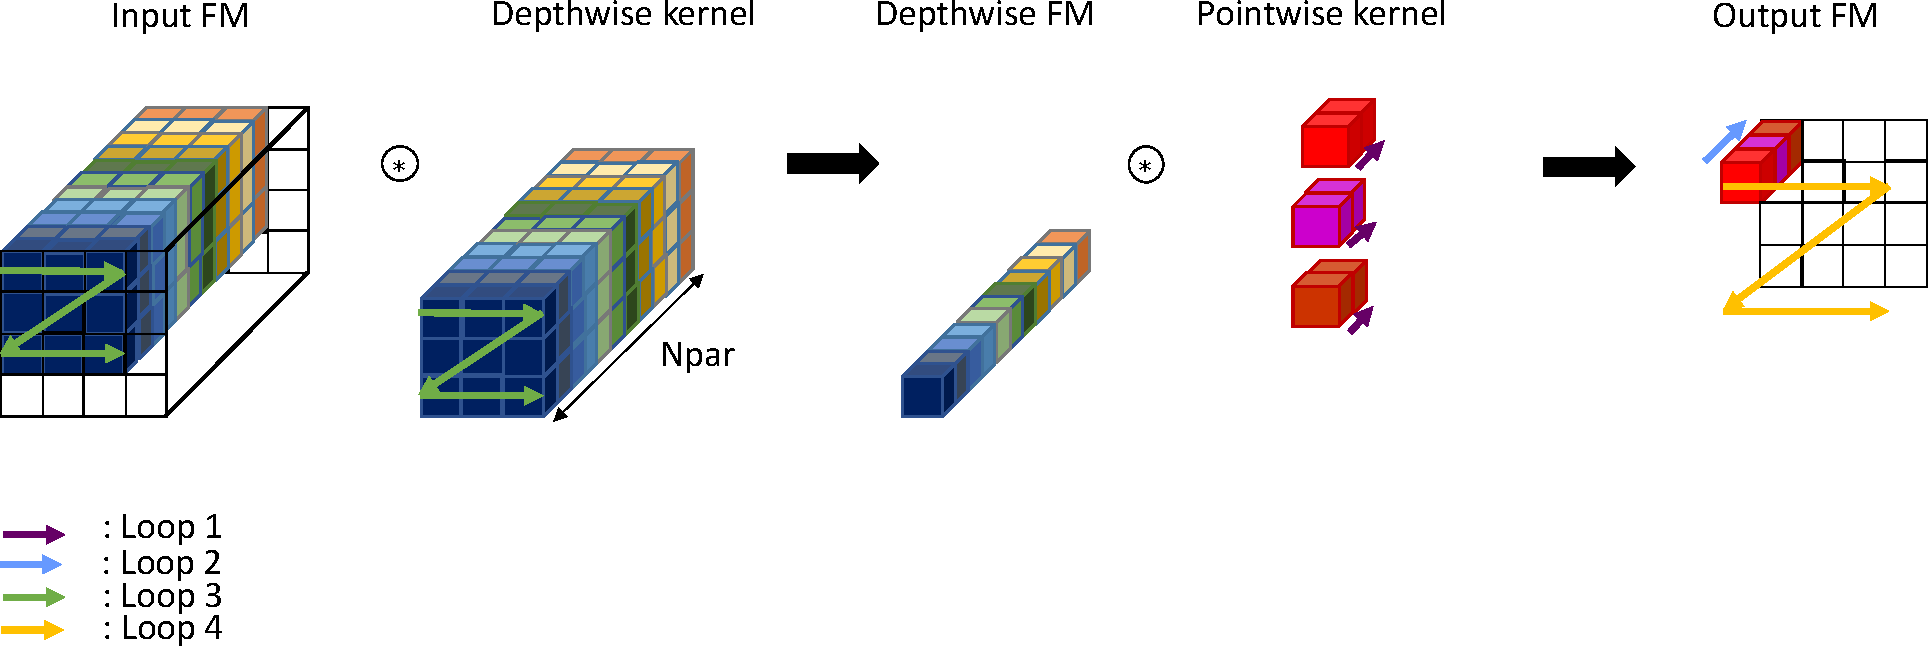
\includegraphics[width=\linewidth]{algo_dsc.pdf}
        \caption{Representation of the sparse \acrshort{dsc} convolution}
        \label{fig:algo_dsc}
    \end{figure}
\end{enumerate}
%
\subsection{Loop analysis}
%
We have determined how the bottleneck convolution is going to be performed. Now we define how it will be implemented on \acrshort{fpga}. As explained in Section \ref{sec:opti_dataflow}, the \acrshort{cnn} inference is executed in three steps:
%
\begin{enumerate}
    \item The \acrshort{fpga} loads a tile of the data from the external memory into the on-chip memory.
    \item The \acrshort{pe}s of the \acrshort{fpga} fetch data from the on-chip memory, use them to perform convolution, and store the computed result into the on-chip memory.
    \item Once the tile of output results is produced, it is stored into the external memory. Either the \acrshort{fpga} loads the next tile and restarts the previous steps, or it stops if the last tile of data has been convolved.
\end{enumerate}
%
If we look at Algorithms \ref{pseudocode:c11} and \ref{pseudocode:dsc}, each convolution is implemented with various levels of loops, named \textbf{convolution loops}. To optimize these operations, three main loop optimization techniques can be used, as presented in Section \ref{sec:opti_dataflow}: loop tiling, loop unrolling, and loop interchange. Those loop optimization techniques include hardware design parameters that define the acceleration factor and hardware footprint \cite{ma_optimizing_2018}. Therefore, we have to analyze the convolution loops to find the optimal tiling, unrolling, and loop interchange parameters. We applied the same methodology as \textcite{ma_optimizing_2018}. However, as they studied the standard convolution, in this work we adapted it to the proposed sparse \acrshort{dsc}.\cite{ma_optimizing_2018}

\textcite{ma_optimizing_2018} identified design objectives to optimize the convolution operation. These following design objectives should be minimized:
%
\begin{itemize}
    \item Partial sum storage.
    \item On-chip memory accesses.
    \item Off-chip memory accesses.
\end{itemize}
%
We will try to minimize them for both $1 \times 1$ and depthwise separable convolution.
%
\subsubsection{Hardware design parameters}
%
Before analyzing the design objectives, we must first define what are the different tiling and unrolling parameters for each convolution. Tables \ref{tab:param_c11} and \ref{tab:param_dsc} define the different dimensions of the volumes and the corresponding hardware design parameters.

\textbf{$1 \times 1$ convolution}: the $1 \times 1$ convolution is composed of three convolution loops (the fourth loop is fully-unrolled according to the algorithm). During Loop-1, we get each fetching group and we do the convolution between them. Loop-1 is determined by the number of input and weight fetching groups (they are the same since otherwise there would be misalignment). The purpose of Loop-1 is to compute the final output result of the convolution. Loop-2 slides spatially the kernel over the input \acrshort{fm} to produce one channel of the intermediate \acrshort{fm}. Since the spatial size of each kernel is $1 \times 1$, there is no spatial reduction between the input and intermediate \acrshort{fm}. The purpose of Loop-3 is to choose which of the required $N_{par}$ intermediate \acrshort{fm} channels is produced.
%
\begin{table}[H]
    \centering
    \begin{tabular}{c|c|c|c}
    \hline \hline
    & \makecell{\# of weight \\ and input \\ fetching group} & \makecell{Input \acrshort{fm} \& \\ intermediate \acrshort{fm} \\ Spatial Axis} & \makecell{intermediate \acrshort{fm} \\ channels} \\
    \hline
    Convolution Loops & Loop-1 & Loop-2 & Loop-3 \\
    Convolution Dimensions & $N_{gr}$ & $N_{ix}$,$N_{iy}$ & $N_{par}$ \\
    Loop Tiling            & $T_{gr}$ & $T_{ix}$,$T_{iy}$ & $T_{intf}$ \\
    Loop Unrolling         & $P_{gr}$ & $P_{ix}$,$P_{iy}$ & $P_{intf}$ \\
    \hline \hline
    \end{tabular}
    \caption{$1 \times 1$ convolution loop dimensions and hardware design variables, inspired by \cite{ma_optimizing_2018}}
    \label{tab:param_c11}
\end{table}
%
\textbf{\acrshort{dsc}}: the \acrshort{dsc} is composed of four convolution loops. Two loops are specific to the depthwise convolution, one to the pointwise convolution, and one loop is shared between the two convolutions. As presented in Section \ref{subsec:mbnv2-pr}, the pointwise convolution uses the results of the depthwise convolution to produce $N_{of}$ partial results to avoid reperforming the same $1 \times 1$ and depthwise convolutions. Loop-1, therefore, aims at looping over the output channels. The depthwise convolution is composed of two loops. Loop-2 performs the 2D convolution between the input channel and the corresponding kernel and Loop-3 loops over the input channel. Finally, Loop-4 is the one that selects which output pixels to compute and fetches the associated input pixels chunk of data from the on-chip memory.
%
\begin{table}[H]
    \centering
    \begin{tabular}{c|c|c|c|c|c}
    \hline \hline
    & \makecell{Output \acrshort{fm} \\ channels} & \makecell{Pointwise \\ kernel size} & \makecell{Intermediate\\\acrshort{fm} channels} & \makecell{Intermediate \acrshort{fm} \\ Spatial Axis} & \makecell{Output \acrshort{fm} \\ Spatial Axis} \\
    \hline
    \makecell{Convolution \\ Loops}      & Loop-1   & Loop-2            & Loop-3     & Loop-4            & Loop-4 \\
    \makecell{Convolution \\ Dimensions} & $N_{of}$ & $N_{kx}$,$N_{ky}$ & $N_{par}$  & $N_{ix}$,$N_{iy}$ & $N_{ox}$,$N_{oy}$\\
    \makecell{Loop \\ Tiling}            & $T_{of}$ & $T_{kx}$,$T_{ky}$ & $T_{intf-dw}$ & $T_{ix}$,$T_{iy}$ & $T_{ox}$,$T_{oy}$\\
    \makecell{Loop \\ Unrolling}         & $P_{of}$ & $P_{kx}$,$P_{ky}$ & $P_{intf-dw}$ & $P_{ix}$,$P_{iy}$ & $P_{ox}$,$P_{oy}$\\
    \hline \hline
    \end{tabular}
    \caption{\acrshort{dsc} loop dimensions and hardware design variables, inspired by \cite{ma_optimizing_2018}}
    \label{tab:param_dsc}
\end{table}
%
\subsubsection{Partial Sum Storage}
%
\textbf{$1 \times 1$ convolution}: to minimize the partial sum storage, we have to keep all partial results in the registers. If we store those partial results into the on-chip or off-chip memory, memory accesses will be less efficient. The optimal solution would be to fully unroll Loop-1. However, two problems arise. First, since the \acrshort{fpga} has constrained resources, it could not be feasible on the target platform. Second, the number of fetching groups vary across the layers since it depends on the number of input channels ($N_{gr} = \frac{N_{if}}{N_{par}}$). We should adjust the unrolling parameter $P_{gr}$ to the worst case and there would be inefficiency problems. Indeed, if $N_{gr} < P_{gr}$, some \acrshort{pe} would not be used. A better solution would be to fully buffer each fetching group and keep the partial results in the registers. Therefore, we should compute Loop-1 first (otherwise some results would be stored in the on-chip memory).
In summary, the number of partial sums is determined by the number of parallel $1 \times 1$ convolution \acrshort{pe}s, as shown in Equation \eqref{eq:psum_c11}. Each $1 \times 1$ convolution \acrshort{pe} can operate in parallel $P_{gr}$ fetching groups. To minimize the storage of partial sum, we should add the following constraint $T_{gr} = N_{gr}$. Moreover, the ratio of $P_{gr}$ to each $N_{gr}$ of the network should be an integer to avoid these inefficiency problems.
%
\begin{equation}
    \# psum_{1 \times 1} = P_{ix} \times P_{iy} \times P_{intf}
    \label{eq:psum_c11}
\end{equation}

\textbf{\acrshort{dsc}}: we can find two kinds of partial sum: the partial depthwise results and the partial output results. According to the proposed algorithm, we can not keep the partial output results in the registers since we produce from each intermediate fetching group all possible partial output results ($T_{of} = N_{of}$). It means that we must keep the tile of output \acrshort{fm} in the on-chip memory as partial results, as illustrated in Equation \eqref{eq:psum_o_dsc}. Since the kernel size is small and constant across the network, we can fully unroll Loop-2 and set $P_{kx} = T_{kx} = N_{kx}, P_{ky} = T_{ky} = N_{ky}$. This approach was also chosen by \textcite{motamedi_placid_2017}. We can also fully unroll Loop-3 $P_{intf-dw} = T_{intf-dw} = N_{par}$, since the fetching group size $N_{par}$ is up to the programmer. As the depthwise convolution is fully unrolled, we can determine the number of depthwise partial sums using equation \eqref{eq:psum_dw_dsc}.
%
\begin{equation}
    \# psum_{DSC_{PW}} = T_{ox} \times T_{oy} \times T_{of}
    \label{eq:psum_o_dsc}
\end{equation}
%
\begin{equation}
    \# psum_{DSC_{DW}} = N_{kx} \times N_{ky} \times N_{par}
    \label{eq:psum_dw_dsc}
\end{equation}
%
\subsubsection{On-chip memory accesses}
%
According to \textcite{ma_optimizing_2018}, the number of on-chip accesses is determined by Equation \eqref{eq:onchipaccess}, where $\#read_{px}$ (resp. $\#read_{wg}$) is the number of reads accesses in the on-chip memory for input pixel (resp. weight), $\#read\_write\_psum$ is the number of write and read accesses if we store the partial sums in the on-chip memory, and  $\#write\_px$ is the number of accesses to write the output results (which is equal to the number of output pixels). Therefore, to reduce on-chip memory accesses, we must limit partial sums stored in on-chip memory and limit the number of reads.
The number of reads can be reduced by reusing the data in the registers and can be expressed using Equation \ref{eq:read_on_px} and \ref{eq:read_on_wg} \cite{ma_optimizing_2018}, where $N_{op}$ is the total number of operations in a convolution. We can analyze for each convolution $Data\_Reuse_{px}$ and $Data\_Reuse_{wg}$.
%
\begin{multline}
    \#On\_chip\_accesses = \#read_{px} + \#read_{wg} + \\ \#read\_write\_psum + \#write\_px
    \label{eq:onchipaccess}
\end{multline}
%
\begin{equation}
    \#read_{px} = \frac{N_{op}}{Data\_Reuse_{px}}
    \label{eq:read_on_px}
\end{equation}
%
\begin{equation}
    \#read_{wg} = \frac{N_{op}}{Data\_Reuse_{wg}}
    \label{eq:read_on_wg}
\end{equation}

\textbf{$1 \times 1$ convolution}: data reuse should be maximized to limit the number of on-chip memory accesses which are less efficient than register accesses. \textcite{ma_optimizing_2018} define two kinds of data reuse: spatial reuse (how many data are reused in one cycle) and temporal reuse (if a data can be reused in more than one cycle). Temporal data reuse is only possible if we compute Loop-2 first (we keep the same kernel for the pixels of a channel). However, since we compute Loop-1 first, this is not possible. To increase spatial data reuse, we must increase the parallelization and so the unrolling parameters, as illustrated in Equation \eqref{eq:px-d-reu} and \eqref{eq:wg-d-reu}, where $Data\_Reuse_{px}$ (resp. $Data\_Reuse_{wg}$) is the data reuse for input pixels (resp. weight).
%
\begin{equation}
    Data\_Reuse_{px - 1 \times 1} = P_{intf}
    \label{eq:px-d-reu}
\end{equation}
\begin{equation}
    Data\_Reuse_{wg - 1 \times 1} = P_{ix} \times P_{iy}
    \label{eq:wg-d-reu}
\end{equation}

\textbf{\acrshort{dsc}}: since Loop-3 and Loop-2 are fully unrolled, we have full temporal data reuse for depthwise weights. The data reuse for pixel and weight for the depthwise convolution can be found in Equation \eqref{eq:px_dw-d-reu} \cite{ma_optimizing_2018} and \eqref{eq:wg_dw-d-reu}. For the pointwise convolution, we can avoid reading input pixels from on-chip memory if we keep the $N_{par}$ results of the depthwise convolution in registers.
Using the same methodology as for \textbf{$1 \times 1$ convolution}, the weight data reuse can be expressed using Equation \eqref{eq:wg_pw-d-reu}
%
\begin{equation}
    Data\_Reuse_{px - dsc} = \frac{N_{kx} \times N_{ky} \times N_{par} \times P_{intx} \times P_{inty}}{\left( \left( P_{intx} - 1 \right)S + N_{kx} \right) \times \left( \left( P_{inty} - 1 \right)S + N_{ky} \right)}
    \label{eq:px_dw-d-reu}
\end{equation}
\begin{equation}
    Data\_Reuse_{wg-dw} = N_{kx} \times N_{ky} \times N_{par}
    \label{eq:wg_dw-d-reu}
\end{equation}
\begin{equation}
    Data\_Reuse_{wg-pw} = P_{ox} \times P_{oy}
    \label{eq:wg_pw-d-reu}
\end{equation}
%
\subsubsection{Off-chip memory accesses}
%
In the model presented in Section \ref{subsec:loopopti}, as the on-chip memory is not large enough to store the whole \acrshort{cnn} size, this one is stored in external memory. However, accesses to external memory are more expensive in terms of latency and energy. Therefore, we should limit the number of off-chip memory accesses per pixel and weight. Instead, we tile the weights and input \acrshort{fm} that we store in the on-chip memory. Once the tile has been fully used, we can load the next tile until the convolution is done.

Since we store every pixel fetching group in the on-chip memory, each pixel is loaded only once from the external memory. However, thanks to padding and the 2D convolution, the input \acrshort{fm} tile can be expressed as Equation \eqref{eq:tileo} \cite{ma_optimizing_2018}. If the input \acrshort{fm} tile does not cover the spatial size of the input \acrshort{fm}, some pixels are included in multiple tiles due to the depthwise convolution, as illustrated in Figure \ref{fig:tilei}. However, it does not concern every pixel. Therefore, we can express the number of external memory accesses per pixel as Equation \eqref{eq:dram_px}.
%
\begin{equation}
    T_{ix/iy} = \left( T_{ox/oy} - 1\right) S + P_{kx/ky}
    \label{eq:tileo}
\end{equation}
\begin{equation}
    \#DRAM\_px = 1
    \label{eq:dram_px}
\end{equation}
%
\begin{figure}[H]
    \centering
    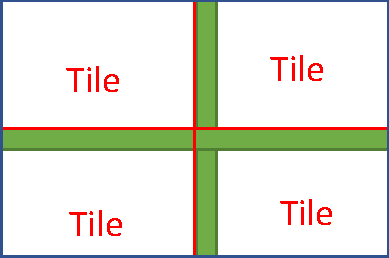
\includegraphics[width=0.6\textwidth]{Tile.pdf}
    \caption{Tiling process on an input \acrshort{fm}, where the green area is the input pixels that would be loaded more than once due to 2D convolution}
    \label{fig:tilei}
\end{figure}
%
If all the weights are not buffered into the on-chip buffer, we have to load from external memory the weight corresponding to the intermediate \acrshort{fm} fetching group. It means that we must fetch each weight every time a new output tile is produced. Therefore, the number of weight external memory access is expressed as Equation \eqref{eq:dram_wg}.
%
\begin{equation}
    \#DRAM\_wg = \frac{N_{ox} \times N_{oy}}{T_{ox} \times T_{oy}}
    \label{eq:dram_wg}
\end{equation}
%
\subsubsection{Summary}
%
After having analyzed the convolution loop, we determined the unrolling and tiling hardware design parameters:
\begin{itemize}
    \item Loop interchange: for both convolutions, we do the loops in the given order (first Loop-1, ..., and then Loop-n).
    \item Loop Tiling: as explained previously, the following tiling parameters are set:
    \begin{itemize}
        \item $T_{gr} = N_{gr}$
        \item $T_{intf} = N_{par}$
        \item $T_{intf-dw} = N_{par}$
        \item $T_{of} = N_{of}$
        \item $T_{kx} = N_{kx}$
        \item $T_{ky} = N_{ky}$
    \end{itemize}
    The other tiling parameters should be set as close as $N_{*}$ (depending on the target platform). Moreover, as pointed out by \textcite{ma_optimizing_2018}, the following constraint should be added to avoid inefficiency: \textquote{$T_{*}$ should be a divisor of $N_{*}$}. Indeed, the \acrshort{pe}s are configured to execute a full tile. If the constraint is not satisfied, some \acrshort{pe}s would not be used.
    \item Loop Unrolling: as explained previously, the following unrolling parameters are set:
    \begin{itemize}
        \item $P_{kx} = N_{kx}$
        \item $P_{ky} = N_{ky}$
        \item $P_{intf-dw} = N_{par}$
    \end{itemize}
    The other unrolling parameters should be set as close as $T_{*}$ (depending on the target platform). Moreover, as pointed out by \textcite{ma_optimizing_2018}, the following constraint should be added to avoid inefficiency: \textquote{$P_{*}$ should be a divisor of $T_{*}$}.
\end{itemize}
%% unrolling
